\documentclass[a4paper]{article}
\usepackage{latexsym,amssymb,amsmath,amsbsy,amsopn,amstext,xcolor,multicol}
\usepackage{ctex,hyperref,graphicx,wrapfig,fancybox,listings}
\usepackage{pgf,pgfarrows,pgfnodes,pgfautomata,pgfheaps,pgfshade}
\usepackage[top=1in, bottom=1in, left=1.25in, right=1.25in]{geometry}
\graphicspath{{pic/}}
\title{\bf 电子学基础第一次仿真作业报告}
\date{2017.11.24}
\author{计64~翁家翌~2016011446}
\begin{document}
\kaishu
\ttfamily
\maketitle
%\tableofcontents
%\newpage
\section{A-1求电路等效电阻}
\subsection{问题叙述}
利用合适的仿真方法,求题图中每个电路的等效电阻。
\subsection{仿真环境}
circuitlab在线仿真:\url{https://www.circuitlab.com}
\subsection{仿真方法}
在所求电路接口接入直流电流,仿真时测量干路电压,以$R=\frac{U}{I}$计算出等效电阻。
\subsection{仿真结果}
\subsubsection{A-1(a)}
\begin{figure}[htp]
\centering
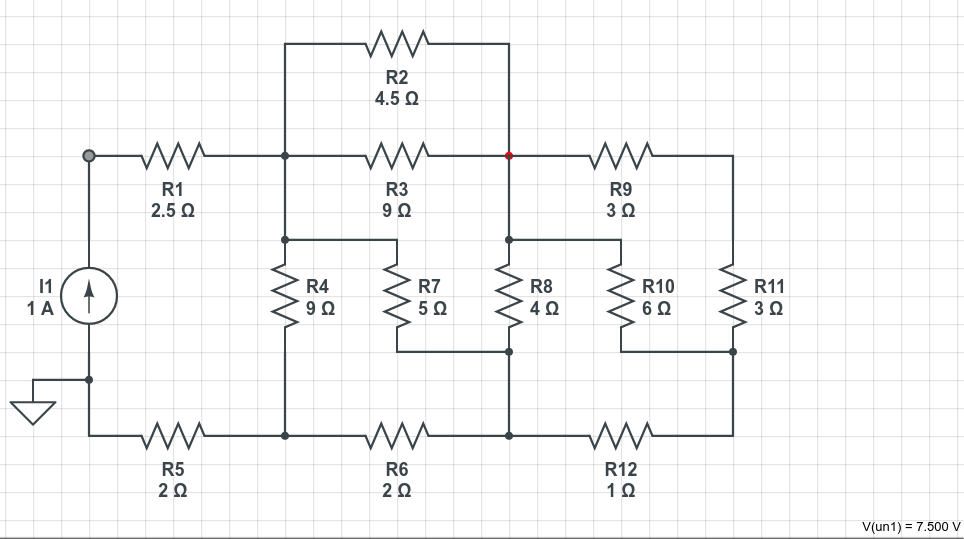
\includegraphics[width=1\linewidth]{A1.png}
\caption{电流源1A,电压7.500V(图中右下角),计算得等效电阻7.500Ω。}
\label{A1a}
\end{figure}
\subsubsection{A-1(b)}
\begin{figure}[htp]
\centering
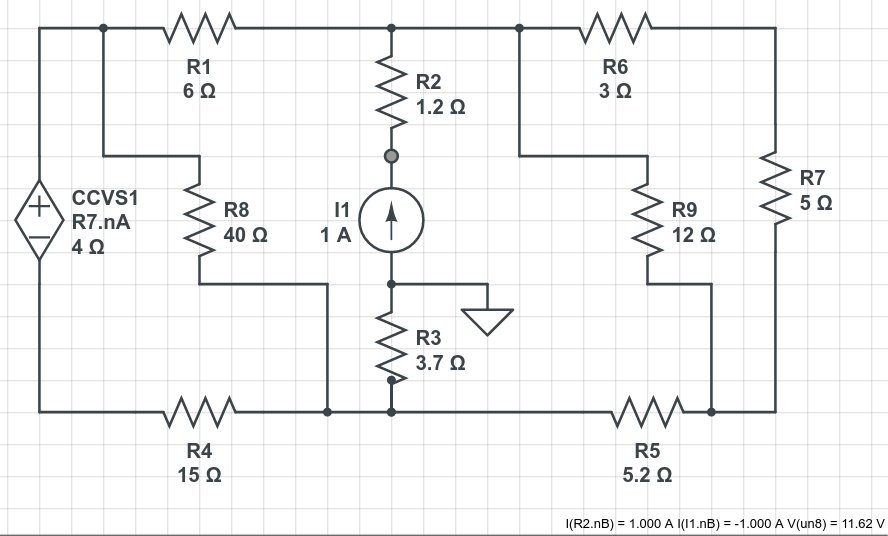
\includegraphics[width=1\linewidth]{A2.png}
\caption{电流源1A,电压11.62V,计算得等效电阻11.62Ω。}
\label{A1b}
\end{figure}

\section{A-4观察交流电路中电容电压}
\subsection{问题叙述}
已知电压信号,同时观察信号源和电容上的电压波形,比较二者区别并说明原因。
\subsection{仿真环境}
circuitlab在线仿真:\url{https://www.circuitlab.com}
\subsection{仿真方法}
在所求电路信号源与电容上连接示波器以显示电压。
\subsection{仿真结果}
\begin{figure}[htp]
\centering
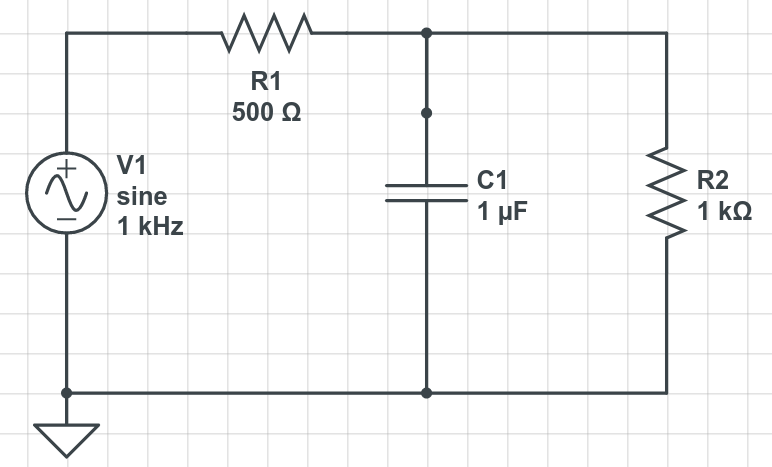
\includegraphics[width=1\linewidth]{A4.png}
\caption{A4电路图}
\label{A41}
\end{figure}

\begin{figure}[htp]
\centering
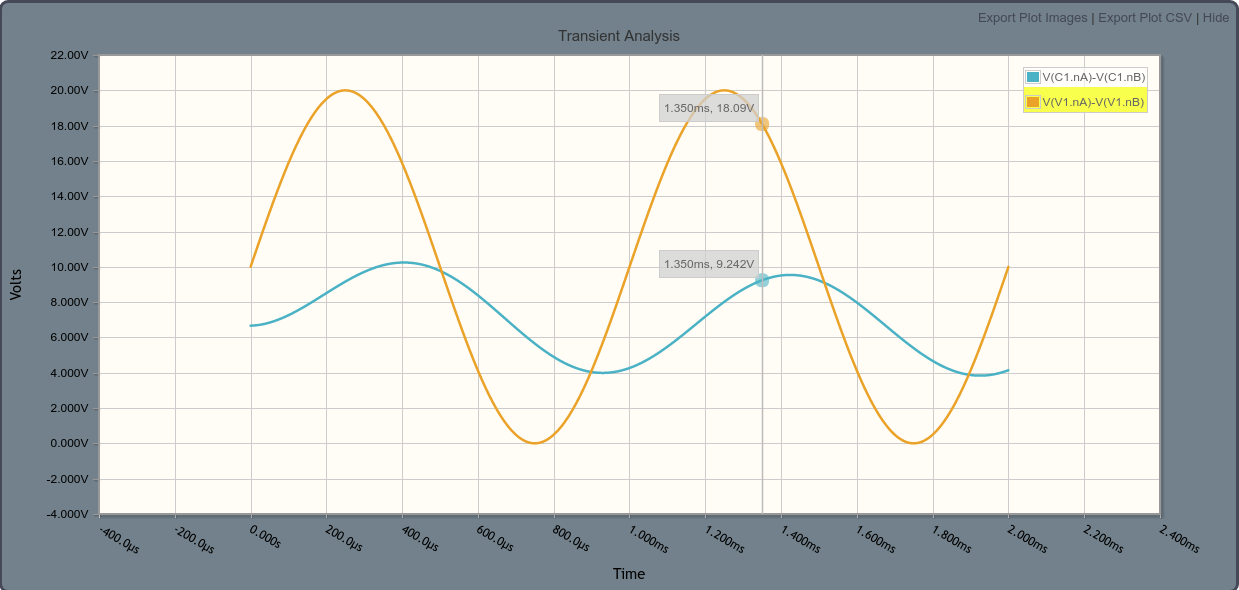
\includegraphics[width=1\linewidth]{A4-2.png}
\caption{振幅较小的为电容电压波形,较大的为信号源波形。二者不同相,电容的存在会使电压落后于电流}
\label{A42}
\end{figure}
\end{document}
